\documentclass[11pt,a4paper]{article}
\usepackage{fontspec}
\setmainfont{DejaVu Serif}
\usepackage{amsmath,amssymb,graphicx,booktabs,geometry,hyperref}
\geometry{margin=22mm}
\sloppy
\setlength{\emergencystretch}{3em}
\begin{document}
\title{Експеримент 5: офсети, градієнти й топологія}\author{}\date{2026-11-01}\maketitle

\section*{Диференціальні метрики}
Для компактної суми похідна обчислюється аналітично:
\[
 \nabla f(x)=\sum_j a_j\phi'(\|x-c_j\|/r)
 \frac{x-c_j}{r\|x-c_j\|}.
\]
У центрах внесок дорівнює нулю за границею.
Еталонні похідні SDF оцінено центральними різницями з кроками
$10^{-5}$ і $2\cdot10^{-5}$. Залишено точки, де різниця градієнтів
менша $10^{-4}$ і норма відрізняється від одиниці менш ніж на $10^{-4}$.
Це чисельна маска локальної регулярності, не аналітичний опис
усієї медіальної осі. Точки --- незалежні Sobol, маска й кількість
виключених записані. Для grid-методів похідні беруться різницями
$10^{-5}h$, тому їхня похибка включає цю апроксимацію.
\[
 E_g=\sqrt{\operatorname{mean}\|\nabla f-\nabla d\|^2},\quad
 E_{eik}=\sqrt{\operatorname{mean}(\|\nabla f\|-1)^2}.
\]
Також виміряно середній косинус напряму нормалі.

\section*{Дискретизація й топологія}
Поля фіксовані після добору; при зміні роздільності не перебудовуються.
Роздільності 2D: $51,101,201$, 3D: $25,41,65$ на вісь.
$H_{sample}$ --- відстань між хмарами вершин дискретних контурів,
а не доведена відстань Гаусдорфа неперервних поверхонь.
Окремо виміряно $|d(x)-t|$ на вершинах модельної поверхні.
Стабілізація трьох чисел є емпіричною перевіркою; збіжність не доведена.

Для foreground обрано 4/6-зв'язність, background 8/26.
З числа компонент $\beta_0$, порожнин $\beta_2$ та характеристики
Ейлера $\chi$ визначається $\beta_1=\beta_0+\beta_2-\chi$ у 3D;
у 2D $\beta_1=\beta_0-\chi$. Перетин межі області позначається
прапорцем; тоді це не топологія необмеженого тіла.
Тонка трубка тора при $t=-0.19$ має радіус лише $0.01$:
навіть 65 точок на вісь можуть не розрізняти її правильно.
\begin{center}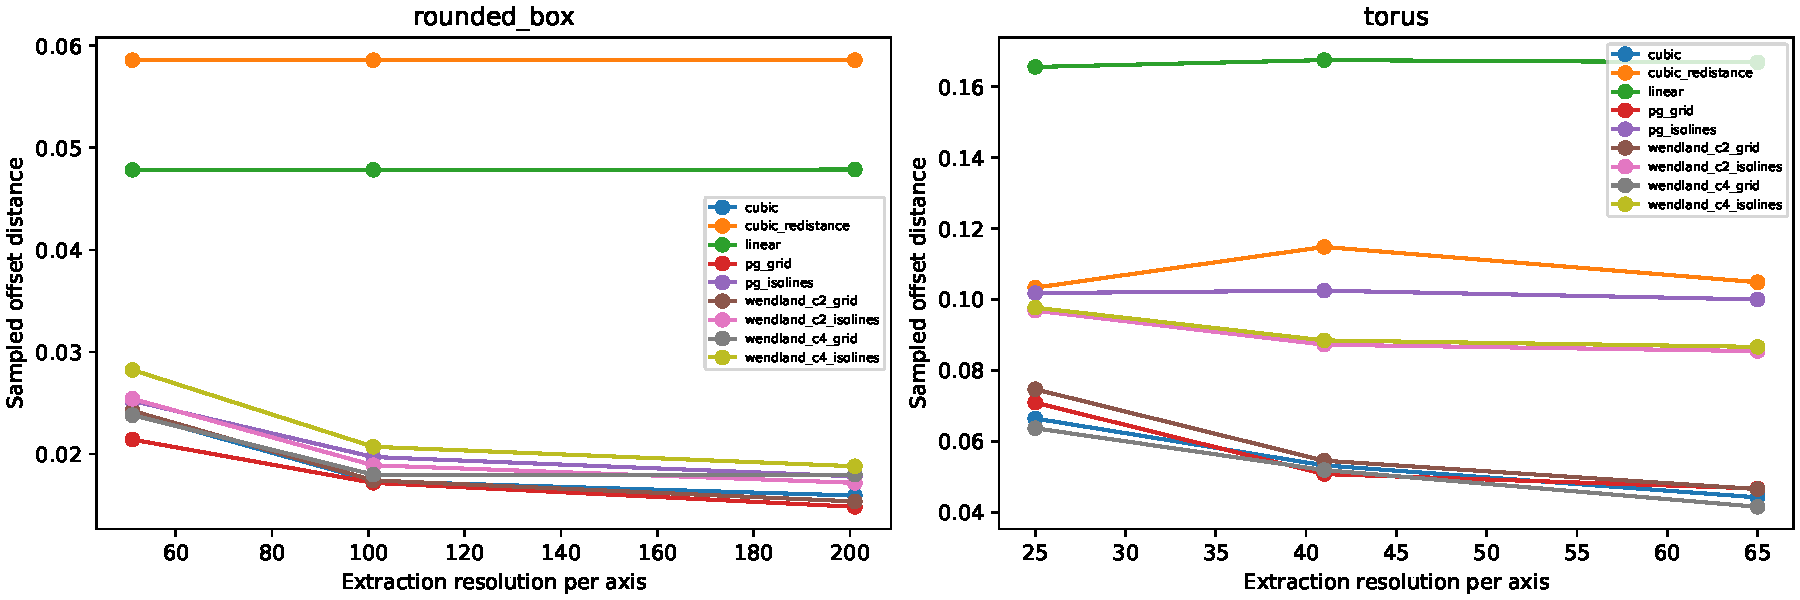
\includegraphics[width=\linewidth]{results/extended/resolution.pdf}\end{center}
\begin{center}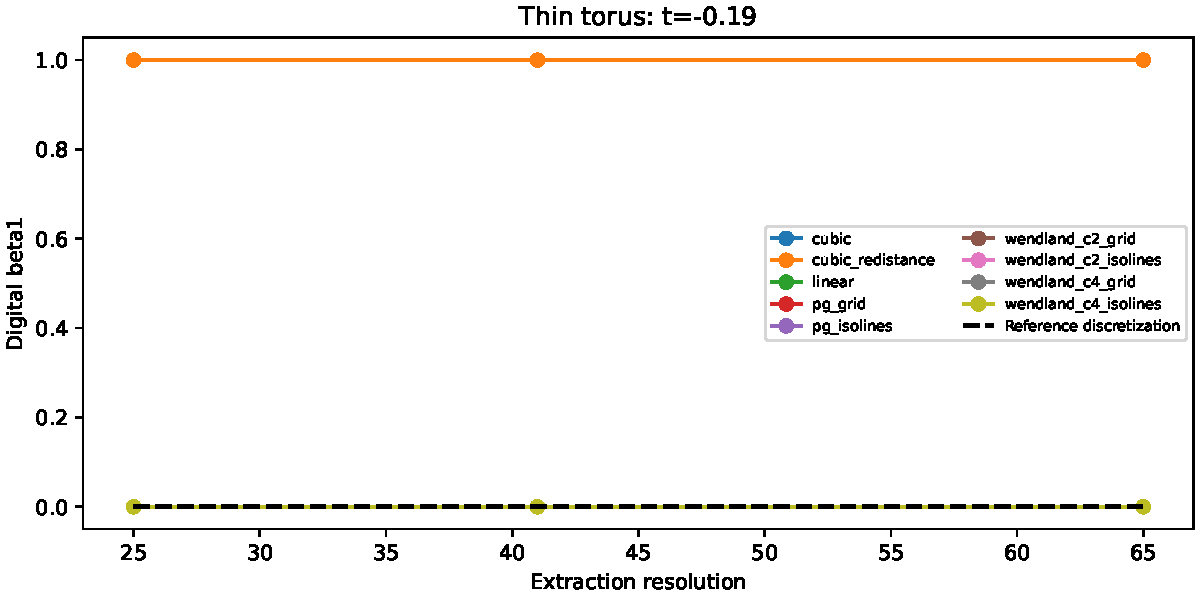
\includegraphics[width=\linewidth]{results/extended/torus_topology.pdf}\end{center}
\begin{center}\small\resizebox{\linewidth}{!}{\begin{tabular}{lllll}\toprule
Метод & $\beta_{1,d}$ & $\beta_{1,f}$ & $H_{sample}$ & $E_g$\\\midrule
pg\_grid & 1 & 1 & 0.04669 & 0.2322\\
pg\_isolines & 1 & 1 & 0.1 & 0.3231\\
wendland\_c2\_grid & 1 & 1 & 0.04652 & 0.2173\\
wendland\_c2\_isolines & 1 & 1 & 0.08544 & 0.2703\\
wendland\_c4\_grid & 1 & 1 & 0.04152 & 0.2169\\
wendland\_c4\_isolines & 1 & 1 & 0.08663 & 0.2785\\
linear & 1 & 1 & 0.1669 & 0.4106\\
cubic & 1 & 1 & 0.04419 & 0.2229\\
cubic\_redistance & 1 & 1 & 0.1049 & 0.9589\\
\bottomrule\end{tabular}}\end{center}
\end{document}
